\documentclass[10pt,a4paper]{article}
% for margining standards
\usepackage[left=3cm,right=3cm,top=3cm,bottom=3cm]{geometry}
% for counting references as a section
\usepackage[numbib,notlof,notlot,nottoc]{tocbibind}
% useful packages
\usepackage{
                graphicx, setspace, fontspec, caption,
                subcaption, float, polyglossia, rotating,
                lscape, pdflscape, indentfirst, tocloft,
                multirow, mathtools, currfile
            }
% paragraph related package
\usepackage[parfill]{parskip}
% use bzar font(THIS MUST BE LOADED BEFORE XePerian PACKAGE)
\setmainfont{BZar.ttf}
% the dear XePersian package
\usepackage{xepersian}
%
% General settings goes here.
%
% lines space
\renewcommand{\baselinestretch}{1.5}
% paragraph first line indention
\setlength{\parindent}{1cm}
% paragraph spacing
\setlength{\parskip}{1em}
% set graphics' path
\graphicspath{ {images/} }
% make table of content dotted
\renewcommand{\cftsecleader}{\cftdotfill{\cftdotsep}}
% define a new command as {half-space} in english
\newcommand{\halfspace}{\hspace{0pt}}
% define a new command as {half-space} in persian
\newcommand{\نیمفاصله}{\halfspace}
% define a shortcut for half-space in general
\renewcommand{\ }{\halfspace}
% define a new command for ease of use for rendering reference
\newcommand{\renderref}[1] { \begingroup \let\clearpage\relax \include{#1} \endgroup }
%
% DOCUMENT BEGIN
%
\begin{document}
\title{
    
\includegraphics[width=0.25\textwidth]{iut}\\\vspace{20pt}
    گزارش تکلیف دوم
}
\author{داریوش حسن\ پور آده}
\date{۹۳۰۸۱۶۴}
\maketitle
\قسمت{قسمت ۱}
در کد ارسالی داده\ ها به صورت گفته شده بارگذاری شده\ اند.
\قسمت{قسمت ۲}
داده\ های آموزشی در دو متغییر $x$ و $\text{\lr{marks}}$ بارگذاری شده\ اند که توسط رابطه\ ی \ref{eq:sec1} وزن\ های بهینه بدست آمد. که وزن\ های بدست آمده به صورت زیر بدست آمده است.
\lr{\[w^* = \begin{bmatrix}
0.30 & 0.30 & 0.05 & 0.05 & 0.15 & 0.15
\end{bmatrix}^T\]}
با توجه به این\ که مجموع وزن\ ها برابر با ۱ می\ باشد می\ توان مقادیر هریک از وزن\ ها را به عنوان درصد اهمیت هریک از ویژگی\ ها که برای محاسبه\ ی نمره\ ی نهایی دانشجویان در نظر گرفته شده است، در نظر گرفت. در نتیجه میزان اهمیت ویژگی\ ها به صورت جدول
\ref{tab:feature_imp_pre}
می\ باشد.
\begin{equation}
w = (x^Tx)^{-1}x^T \cdot \text{\lr{marks}}
\label{eq:sec1}
\end{equation}
\begin{table}
\centering
\begin{latin}
\begin{tabular}{l|c}
Feature & Importance\%\\\hline
midterm & 30\%\\
finalterm & 30\%\\
tak1 & 5\%\\
tak2	 & 5\%\\
research	 & 15\%\\\
project & 15\%
\end{tabular}
\end{latin}
\caption{درصد اهمیت هریک از ویژگی\ ها برای محاسبه\ ی نمره\ ی نهایی}\label{tab:feature_imp_pre}
\end{table}
نمره\ های بدست آمده برای داده\ های تست با استفاده از وزن\ های بدست آمده به صورت جدول
\ref{tab:sec2_test_res}
می\ باشد.
\begin{table}
\centering
\begin{latin}
\begin{tabular}{c|c}
Student\# & Grade\\\hline
1 & 6.80\\
2 & 12.05\\
3 & 17.10\\
4 & 11.60
\end{tabular}
\end{latin}
\caption{جدول نمره\ های پیش\ بینی شده برای داده\ های آموزشی برای قسمت دوم}\label{tab:sec2_test_res}
\end{table}
\قسمت{قسمت ۳}
وزن\ های بدست آمده در این قسمت به صورت زیر می\ باشد.
\lr{\[w^* = \begin{bmatrix}0.27 & 0.34 & 0.09 & 0.07 & 0.16 & 0.08\end{bmatrix}^T\]}
نمودار خطا برحسب تعداد دفعات تکرار را در شکل
\ref{fig:sec2_mse}
آمده است. در یادگیری ضریب یادگیری
\lr{$2e-5$}
 و حداکثر تعداد دوره ۳۰۰ در نظر گرفته شده است. نتایج پیش\ بینی بروی داده\ های تست در جدول
\ref{tab:sec3_test_res} 
آمده است همان\ طور که مشاهده می\ شود نمره\ های بدست آمده در این قسمت نزدیک به مقادیر بدست آمده در جدول
\ref{tab:sec2_test_res}
می\ باشد که نشان می\ دهد الگوریتم نوشته شده درست کار می\ کند. همچنین وزن\ های بدست آمده در این روش با ظریب یادگیری ذکر شده نزدیک به وزن\ های بدست آمده در قسمت قبل می\ باشد.
\begin{figure}[h!]
\centering
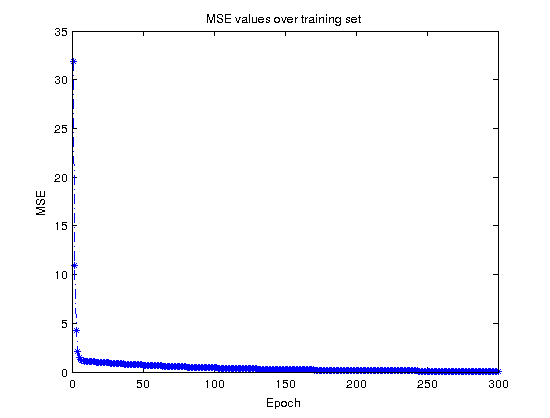
\includegraphics[width=\textwidth]{sec3_mse}
\caption{نمودار خطا برحسب تعداد دفعات تکرار برای قسمت دوم با ضریب یادگیری \lr{$2e-5$}}\label{fig:sec2_mse}
\end{figure}
\begin{table}
\centering
\begin{latin}
\begin{tabular}{c|c}
Student\# & Grade\\\hline
1 & 5.94\\
2 & 10.60\\
3 & 17.59\\
4 & 11.21
\end{tabular}
\end{latin}
\caption{جدول نمره\ های پیش\ بینی شده برای داده\ های آموزشی برای قسمت ۳}\label{tab:sec3_test_res}
\end{table}
در صورتی که ضریب یادگیری را به مقدار
\lr{$2e-4$}
افزایش دهیم نمودار \lr{MSE} و وزن\ های بدست آمده به صورت زیر می\ باشد. همان\ طور که مشاهده می\ شود به این هیچ عنوان خوب یادگرفته نشده است -- چون از به دلیل طول گام بزرگ بهینه\ های محلی/جهانی را رد می\ کند.
\[\hat{w} = \begin{bmatrix}0.30 & 0.30 & 0.05 & 0.05 & 0.15 & 0.15\end{bmatrix}\]
\begin{figure}[h!]
\centering
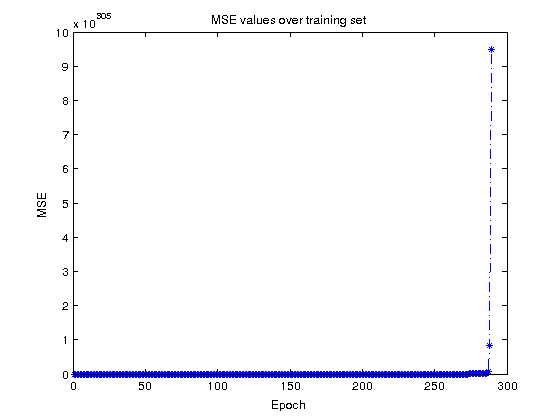
\includegraphics[width=\textwidth]{sec3_mse_lr_2e_4}
\caption{نمودار خطا برحسب تعداد دفعات تکرار برای قسمت دوم با ضریب یادگیری \lr{$2e-4$}}\label{fig:sec2_mse}
\end{figure}
\newpage
در صورتی که با ضریب یادگیری
\lr{$2e-5$}
با تعداد دوره\ ی ۱۰،۰۰۰ بار برنامه را اجرا کنیم ظرایب بدست آمده \textbf{دقیقا} معادل با ظرایب بدست آمده در قسمت ۲ می\ باشد، که نشان می\ دهد با فرصت کافی و ظریب یادیگری مناسب برنامه می\ تواند به بهینه\ ی جهانی همگرا شود.
\newpage
\قسمت{قسمت ۴}
در این قسمت به ازای دانشجویانی که نمره\ ی بالای ۱۲ را گرفته\ اند مقدار ۱ و برای کمتر از ۱۲ را مقدار ۰ به عنوان مقادیر هدف در نظر گرفته شده است. بعد از آموزش وزن\ ها و نتایج حاصل بروی داده\ های تست به صورت زیر می\ باشد.
\lr{\[w_* = \begin{bmatrix}0.02 & 0.05 & -0.02 & 0.01 & 0.00 & 0.00\end{bmatrix}\]}
\begin{table}
\centering
\begin{latin}
\begin{tabular}{c|c|c}
Student\# & Output & {\small Passed(threshhold = 0.5)?}\\\hline
1 & 0.3224 & false\\
2 & 0.7345 & true\\
3 & 0.9509 & true\\
4 & 0.5721 & true
\end{tabular}
\end{latin}
\caption{جدول نمره\ های پیش\ بینی شده برای داده\ های آموزشی برای قسمت ۴}\label{tab:sec4_test_res}
\end{table}
همان\ طور که مشاهده می\ شود نمره دانشجوی شماره\ ی ۴ که در قسمت ۱ زیر ۱۲ پیش\ بینی شده است و مردود به حساب می\ آید در نتایج این قسمت قبول شده است -- که نشان دهنده خطای مدل دسته\ بند بدست آمده است.
\end{document}
